In this chapter we turn to the implementation of the function $G_T$ by discussing a method to learn the function $\Gamma$. We apply our methodology to some chaotic attractors. 
Most notably, we consider the reconstruction of the chaotic attractor of the double pendulum -- an  attractor that has not previously been successfully reconstructed because of its intricate structure. In fact the previous data-driven approaches also have not been successful in building a model from the double pendulum. 

%We then indicate where this implementation differs from previous work done by (\cite{manjunath2021universal}) and empirically show that the SDD of $G_T$ are less functionally complex than $\Phi_{k, \theta}$ or $T$ by considering the Pearson correlation coefficient. Finally, we present and discuss some numerical results for a focus system of this project: the double pendulum. We also consider other chaotic attractors.

\section{Implementing $G_T$}
The map $G_T$ is implemented by applying the functions $\Gamma$, $g$ and the projection function $\pi_2$ in the relevant order as described by the equations~\ref{eqns_from_data}\ednote{How do I get both?}. To reach this point though, one must first learn $\Gamma$.
After first normalising the data to ensure that it has zero mean value, lies within the range $[-1,1]$, and has been zero-padded as required (see paragraph below for further discussion), we drive the system with external input through the function $g$.

From~\eqref{eqn_driving} we recall the equation of the RNN: \[g(u,x) = (1-a) x + a \tanh(Au + \alpha B x).\]
Recall that $g$ is SI-invertible when the matrix $A$ has the same dimension as $B$ and is invertible. We refer to $A$ as the \textit{input} matrix and $B$ the \textit{reservoir} matrix. 

We make use of a Recurrent Neural Network (RNN) in our implementation to project the data on to a higher dimensional space. We do not train the RNN in the ways familiar to literature and opt to follow the methodology of~\cite{manjunath2021universal}. 
A few words about the RNN's: RNN's are widely used in the literature for temporal processing of data as a type of deep learning technique. 
They take the form of equations considered to be discrete-time version of continuous dynamical systems that model a neural network of neurons~\cite{jaeger2001echo}.

We implement a feedforward network (a network with no memory, unlike the RNN) to learn $\Gamma$ in the \emph{Python} programming language and making use of the \emph{Scipy} library, alongside the \emph{Keras} package in the \emph{Tensorflow} library .

If the RNN we will be using has $N$ neurons, then $A$ and $B$ are each $N\times{N}$ matrices. Inputs $u_n$ of dimension $K < N$ are padded by zeroes (as remarked earlier) to embed the input in a space of dimension $N$. 
As we do not need the entire left-infinite history of an input, an arbitrary initialisation of the system with initial values, followed by the driving of the system with the function $g$ will mean that the generated values approach the actual solution elements in a uniform manner. This follows from the UAP that discussed in the preceding chapter (see~\ref{Dfn_UAP} and subsequent discussion).

Thirdly, we prepare the network by setting up a network with $N$ neurons  to obtain successive state values as samples in the space $Y_T$. 
The actual learning of $\Gamma$ is done using the Adam Optimiser where the means square error (MSE) loss function is optimised. 
The system is trained several times (in our case 4) with incrementally smaller learning rates on each run (0.001 and thereafter divided by 10 at each run). 
Additional parameters such as the number of network-layers, neurons per layer and training-length are presented case-by-case below.

Once $\Gamma$ is learnt, we progress to the the prediction step where $u_n$ is forecasted from $(x_{n-1},x_{n})$. Note that  due to causal embedding $(x_{n-1},x_{n})$ is in one-to-one correspondence with the left-infinite orbit $(\ldots,u_{n-1},u_{n-1})$. 
When $u_n$ is computed using $\Gamma$, it is fed to the driven system $g$ along with  $x_n$ to obtain $x_{n+1}$. Now we apply $\Gamma$ on $(x_n,x_{n+1})$ to forecast $u_{n+1}$ and the whole process repeats. Note that this corresponds to implementing the two model equations for learning from data~\eqref{eqns_from_data}.

\section{Delay Coordinates}

We also consider a more general problem of learning an attractor of dynamical system when only observations of an orbit are given. 
Explicitly, if $(W,T)$ is a dynamical system with dynamics generated by $w_{n+1}=Tw_n$, and if $\theta:W \to \mathbb{R}$ is an observable, then the task is to learn a dynamical system that is topologically conjugate to $(W,T)$ and predict $\theta(w_{m+1}),\theta(w_{m+2}),\ldots$ using the data $\theta(w_{0}),\theta(w_{1}),\ldots,\theta(w_{m})$.  

So how do we do it? Suppose the input generated from the delay-coordinate map $\Phi_{\theta,2d}(\theta(w_{n})) := (\theta(w_{n-2d}),\ldots,\theta(w_{n-1}),\theta(w_{n}))$ is such that Takens delay embedding theorem (see Theorem~\ref{Thm_Takens}) holds.
In that case, there exists a homeomorphism  $F_\theta: \Phi_{\theta,2d}(\theta(w_{n})) \mapsto \Phi_{\theta,2d}(\theta(w_{n+1}))$. If we then feed the input values $u_n := \Phi_{\theta,2d}(\theta(w_{n}))$ to a driven system $g$ having SI-invertibility and the USP, the induced system $(Y_F,G_F)$ would be topologically conjugate to the inverse-limit space of
$(\Phi_{\theta,2d}(W), F_\theta)$ due to Theorem~\ref{Thm_CET}, and hence one could forecast the values ($u_n,u_{n+1},\ldots$). 

In summary, one could forecast  the values $\theta(w_n), \theta(w_{n+1}),\ldots$ by feeding these observations as delay coordinates since the input is again an orbit from a dynamical system. 
The advantage of feeding delay-coordinates to a driven system over learning a map that describes the evolution of the delay coordinates is that the embedding is stable in the sense of global dissipativity that we have described in a previous section~\ref{subs_LearnGamma}.
I.e., there is an attractor $A$ of a map that implements $G_T$ on an expansion $Y_F^+$ providing some robustness to noise. 

We now turn our attention to another practical issue related to the forecasting of chaotic dynamical systems.  
Recall that the twin equations~\ref{eqns_from_data} generate a model from data. 
For a chaotic system, a small amount of noise due either to input-noise or computational error would cause solutions from even a very accurate model with the same initial conditions to diverge. %\ednote{Grammarly}
Statistically, however,  a chaotic system will behave well in the sense that the visiting frequency (the average time spent by an orbit in any region of the phase space of the dynamical system) is identical for almost all initial conditions. 
The phrase `almost all' here is specified as a measure and refers to a result in ergodic theory (\cite{wikiErgodicTheory}) which is a topic beyond the scope of this project.
To illustrate the accuracy of the twin  equations~\ref{eqns_from_data} in modelling the data, we plot the densities of the trajectories of the actual and predicted solutions in ~\ref{fig:dp_success_density},~\ref{fig:noisydp_success_density} and ~\ref{fig:Thomas_TrajDensity}.

In our implementation, the input and reservoir  matrices $A$ and $B$ in the RNN are sparse matrices. This sparsity is not essential but seems to perform slightly empirically better than choosing the matrices arbitrarily.  We also discuss three specifics relating to this concept. Firstly, the matrices are assigned a variable density in terms of the amount of non-zero entries and are scaled to have values within the range $[-1,1]$. For this, we make use of \textit{Python's SciPy} library and specifically the \textit{Sparse, LinAlg} modules. In our experiments, we generally opted for a density ratio of 10\%-25\%.
Secondly, we opt to enforce the requirement that both matrices be well-conditioned, i.e. that they have a condition number of 1. The condition number of a matrix $M$ is the product of the matrix norms of the matrix $M$ and its inverse $M^{-1}$ and is a measure of the sensitivity of output of a matrix multiplication when an input is changed.  We do not have any theoretical justifications for this. 

Lastly, we ensure the matrix $B$ has unit spectral radius so that the variable $\alpha$ in the RNN equation \eqref{eqn_driving} can be used to know if the USP is satisfied. 
It is a  feature that a matrix with a spectral radius less than 1 generally has the USP~\cite{yildiz2012re}.  

We remark on one more aspect that helps produce slightly better empirical results.  To learn $\Gamma: (x_{n-1},x_{n}) \mapsto u_n$ through our feedforward network, we could feed the principal components. 
Principal components are used only for a more efficient state representation to possibly reduce learning errors; it is not a lossy approximation since we use all principal components.

More explicitly, denote $X_{1:N}$ as the matrix with the first $N$ states of the network data represented by row vectors. 
$X_{1:N}=U\Sigma P^T$ here represents the singular value decomposition of $X_{1:N}$ ($U$ and $V$ are unitary matrices, and $\Sigma$ is a diagonal matrix) and we refer to \cite{wikiSVdecomp}. 
We then denote the principal component matrix by the symbol $P$, and the principal components are given by 
 $Z_{1:N}=X_{1:N}P$.
These principal components are used to train a feedforward neural network. 

Denoting the row vectors of $Z_{1:N}$ by  $z_i^T, i=1,2,\ldots,N$ and the neural network by $NN$, the network is trained to learn an approximation of the map
$NN: (z_{n-1},z_n) \mapsto  u_n.
$
The learnt approximation of $NN$ can be used to approximate $\Gamma$ because 
\begin{equation}\label{Seq_RNN}
  NN\left( \begin{bmatrix} 
    P^Tx_{n-1} \\
    P^Tx_n
    \end{bmatrix}
    \right) = NN \circ 
    \begin{bmatrix}
    P^T & 0 \\
    0 & P^T 
    \end{bmatrix}\begin{bmatrix}
    x_{n-1}\\
    x_n
    \end{bmatrix} = u_n = \Gamma(x_{n-1},x_n).
\end{equation}


\section{Experimental Results}
In this section we showcase numerical results pertaining to three attractors that were simulated using the theory and described methodology. We first consider a simple physical system that exhibits complicated dynamics.
\subsection{Double Pendulum}

The Double Pendulum consists of two pendulums fastened to one another such that the system moves as a whole. The first (or higher pendulum) is attached to a fixed point while the second is attached to the endpoint of the first. (See Figure~\ref{fig:dp_setup} below.)
This system shows chaos in a striking manner -- consider once more Figure~\ref{fig:dp_sdic}.
The system has four variables: for each pendulum rod an associated angle and angular velocity. An ideal system is assumed where the rods are massless and pivots are frictionless.
\begin{figure}[ht]
  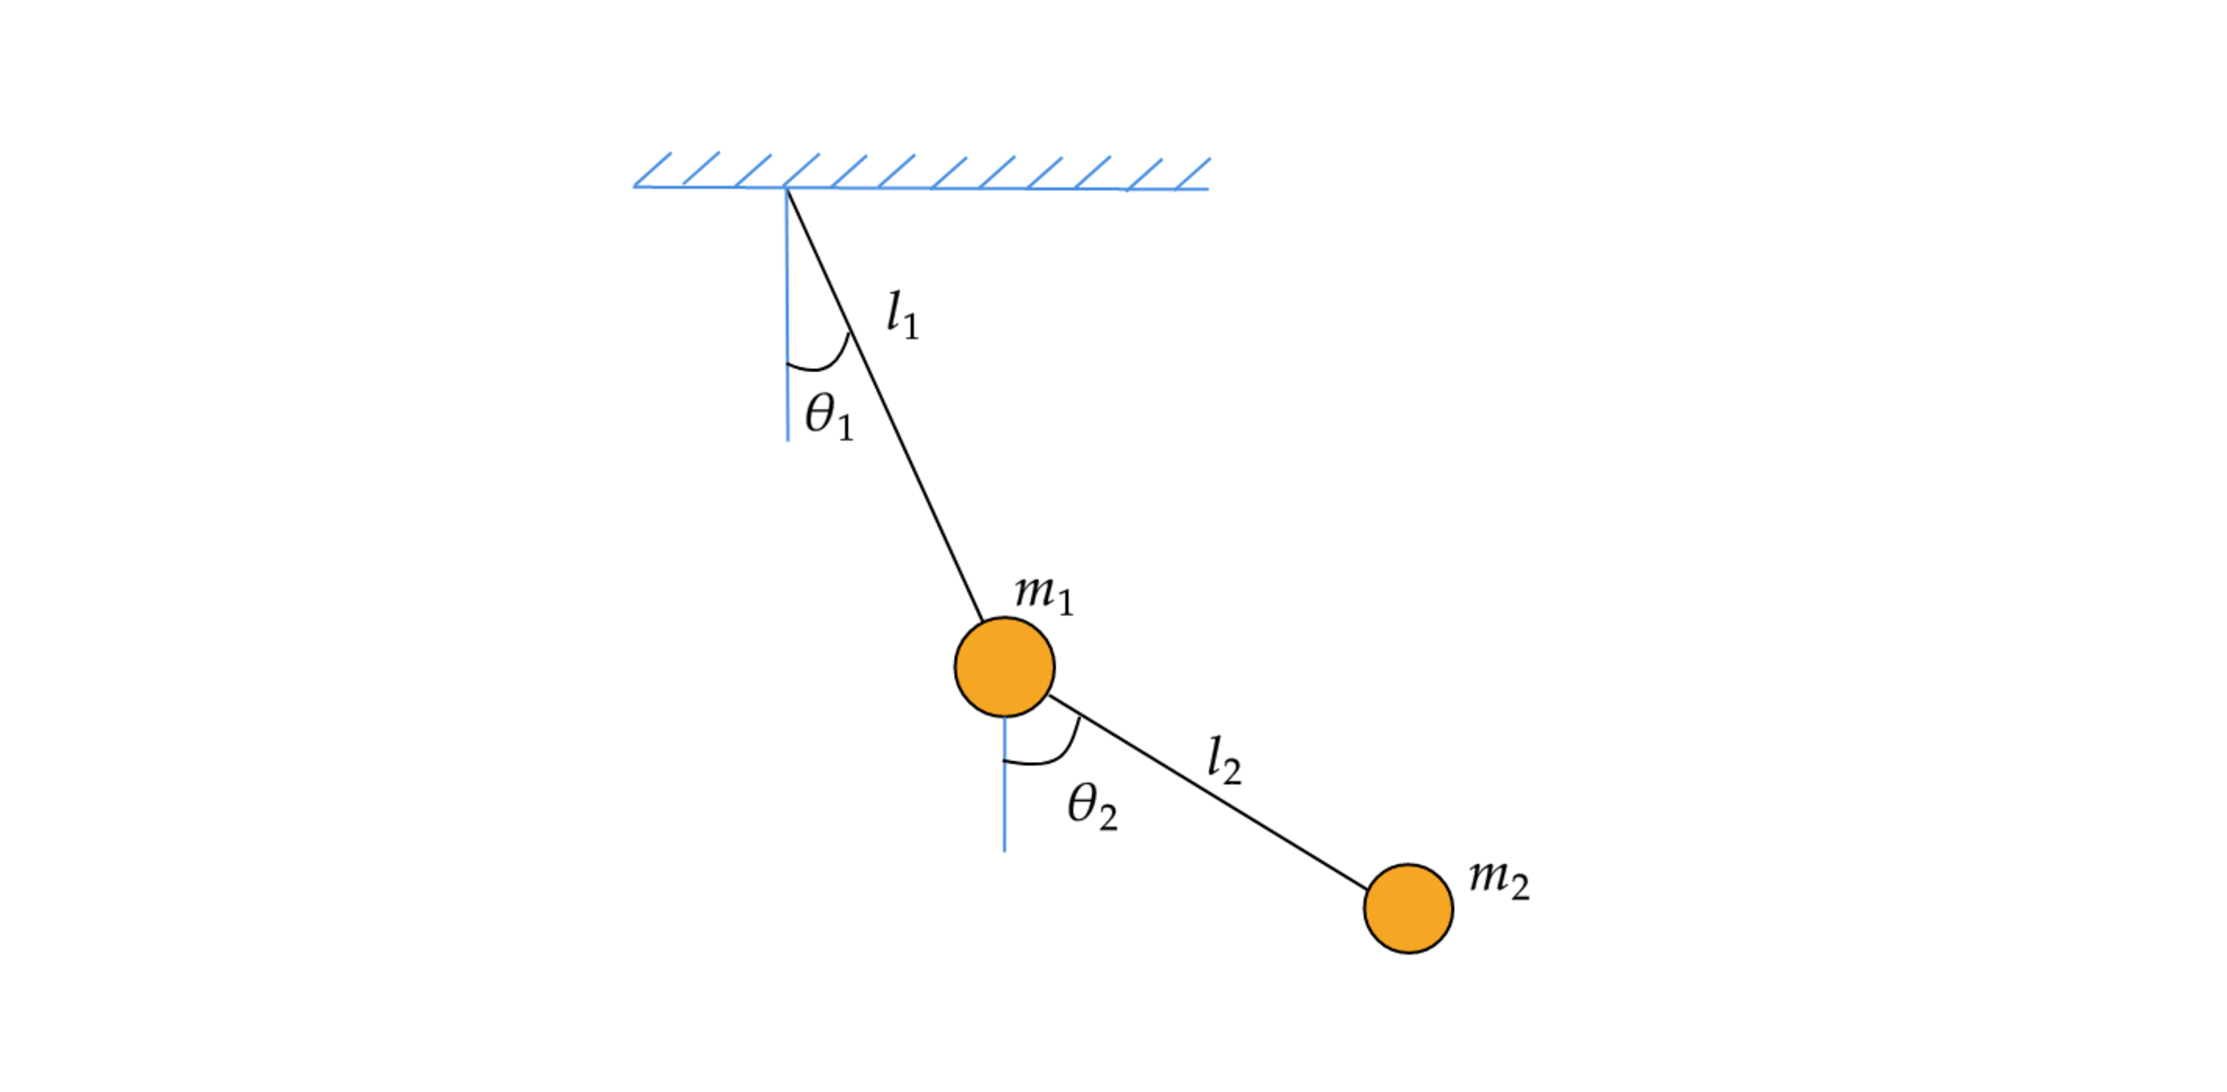
\includegraphics[width=0.8\linewidth]{Graphs/_dp_setup.eps}
  \centering
  \captionof{figure}{Pictorial representation of the setup of a DP where $\theta, m, l$ represent the angle, rod-length, and pendulum head mass respectively.}
\label{fig:dp_setup}
\end{figure}

The scalar equations of motion are derived using Newtonian physics and are reproduced from~\cite{DPFormulas} in Equations~\ref{eqns_dp}. 
Each pendulum component has an associated mass of the head, $m$, and length of the rod, $L_i$. Acceleration due to gravity is denoted by the variable $g$ and initial velocities by $\dot{\theta}$
\begin{eqnarray}\label{eqns_dp}
  \ddot{\theta_{1}}  = \frac{-g(2m_1+m_2)\sin{\theta_1} - m_2g\sin(\theta_1-2\theta_2) - 2\sin(\theta_1-\theta_2)m_2({\dot{\theta_{2}}}^{2}L_2 + {\theta_{1}'}L_1\cos(\theta_1-\theta_2))} {L_1(2m_1 + m_2 -m_2\cos(2\theta_1 - 2\theta_2))}
  \\
  \ddot{\theta_{2}} = \frac{2\sin(\theta_1-\theta_2)(\theta_{1}'^{2}L_1(m_1+m_2) + g(m_1+m_2)\cos\theta_1 + \dot{\theta_{2}}^{2}L_2m_2\cos(\theta_1-\theta_2))}{L_2(2m_1 + m_2 -m_2\cos(2\theta_1 - 2\theta_2))}
\end{eqnarray}

% The second-order system is converted to a first-order ODE system and solved using the Runge-Kutta numerical method.  
Here we chose the values $m_1=2.0$, $m_2=2.0$, $L_1=1.5$ and $m_2=1.5$ with initial velocities $v_1=1.5, v_2=-2$ for the respective pendulum heads.
With a change of variables the second-order system can be written as a system of first order equations with four variables, where each pendulum has an associated $x$ and $y$ coordinates of the mass (the lengthy equations are not shown here). 
The ODE system is then solved using the fourth-order Runge-Kutta numerical method.  

% Undamped DP data-sets were generated and used in this project due to the requirement that the map $T$ be surjective that we must not forget. 
% An example of this would be the case of a DP exhibiting energy-loss (i.e. where the map $T$ is not surjective). In such a case, the attractor is a single point in the phase space when the double pendulum comes to rest. 
% It must be mentioned once again that if we use data outside the attractor, learning is not reliable. 
% To see this, consider Figure~\ref{fig:damped_pendulum} and~\ref{fig:dp_notsurjective}.

We need the assumption of an undamped system so that the map $T$ resulting from the discretization of the system  is surjective.  If we assume, damping surjectivity is lost on any phase space with more than one point.  
An example of this would be the case of a DP exhibiting energy-loss. In such a case, the attractor is a single point in the phase space representing the instant when the double pendulum comes to rest. 
If we use data outside the attractor in this scenario, learning is not reliable. To see this, consider the plots~\ref{fig:damped_pendulum} and~\ref{fig:dp_notsurjective}.

\begin{figure}[ht]
  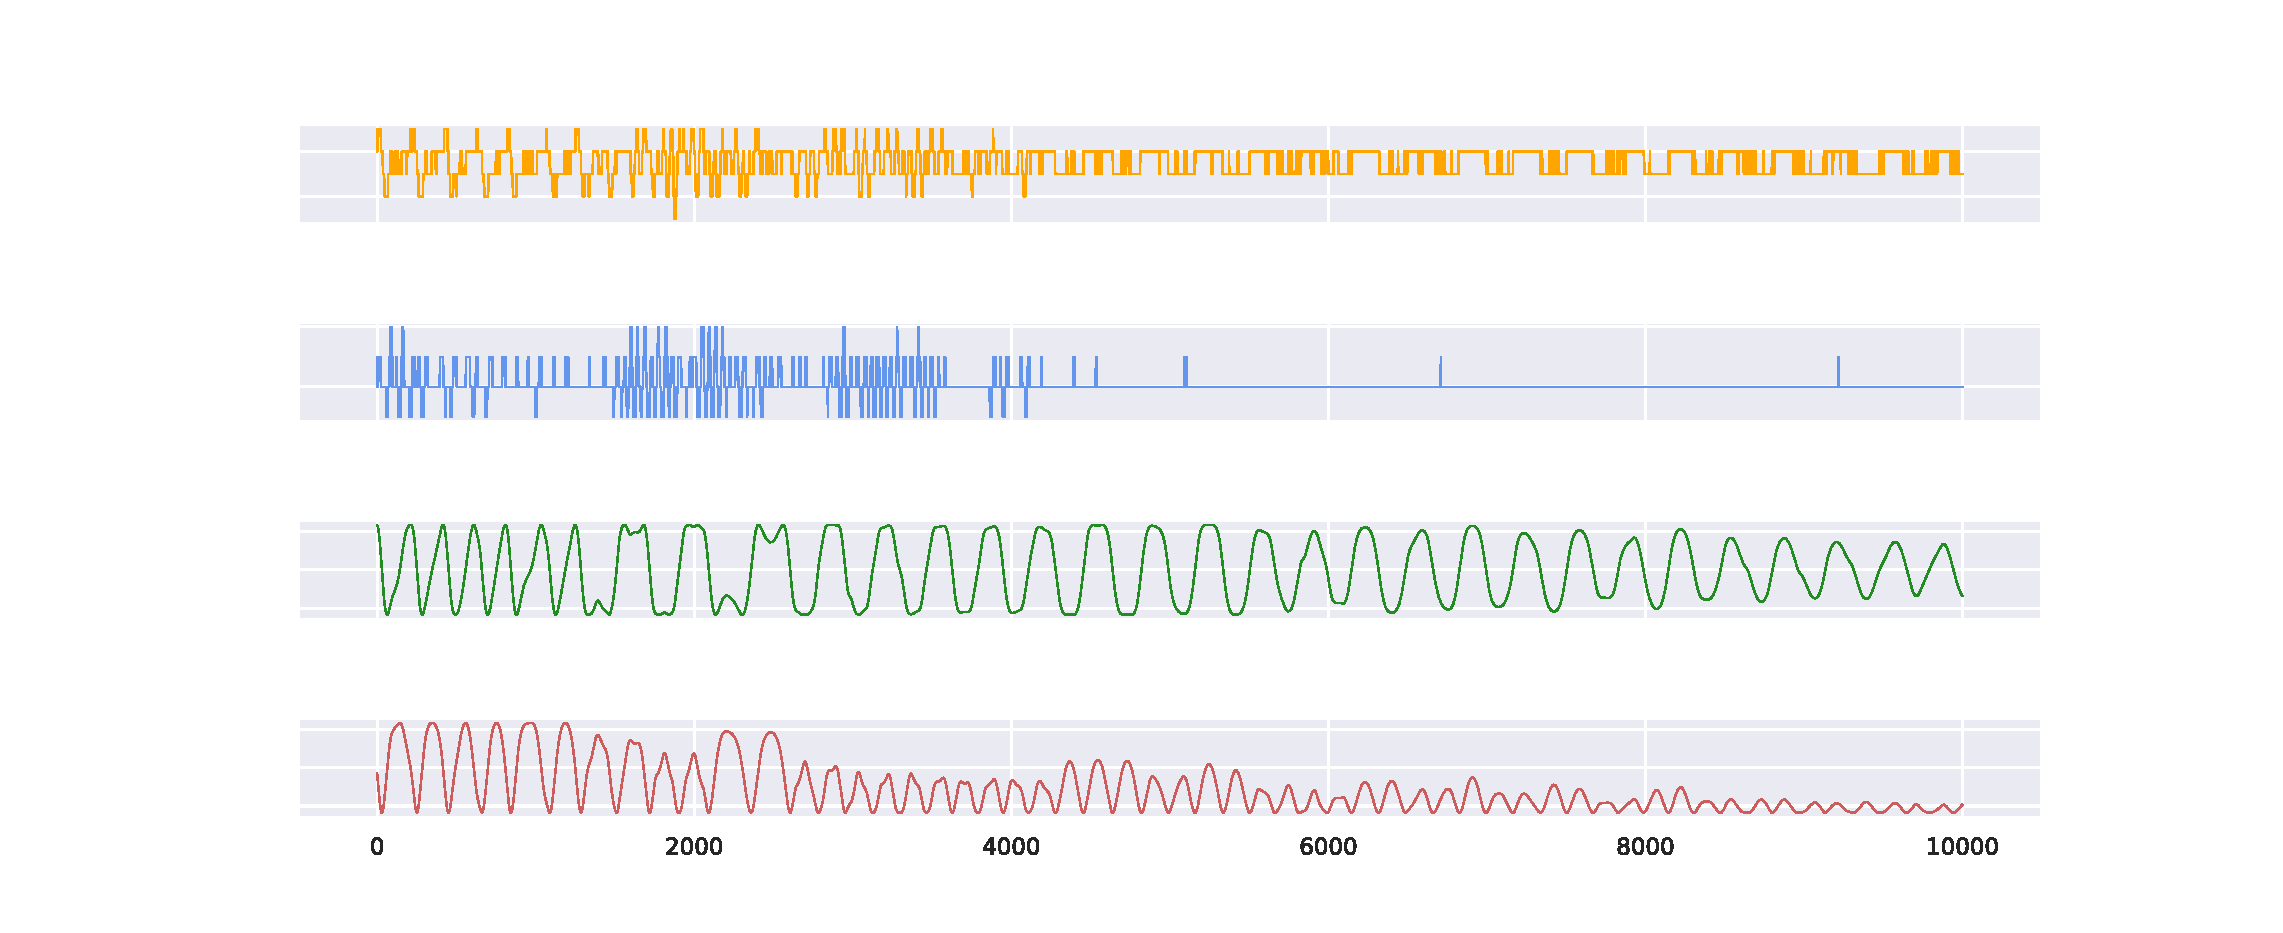
\includegraphics[scale=0.4]{Graphs/_dp_dying.eps}
  \centering
\caption{$x$- and $y$-coordinates of the two pendulum heads plotted for a dataset that exhibits dying oscillations. The map generating the (four-dimensional data) for a damped pendulum is not surjective and so learning $\Gamma$ for this dataset will fail. Consider below the Figure~\ref{fig:dp_notsurjective}. Data obtained from chaotic double pendulum dataset generated from videos takes of experimental pendulums~\cite{asseman2018learning}}
\label{fig:damped_pendulum}
\end{figure}

\begin{figure}[ht]
  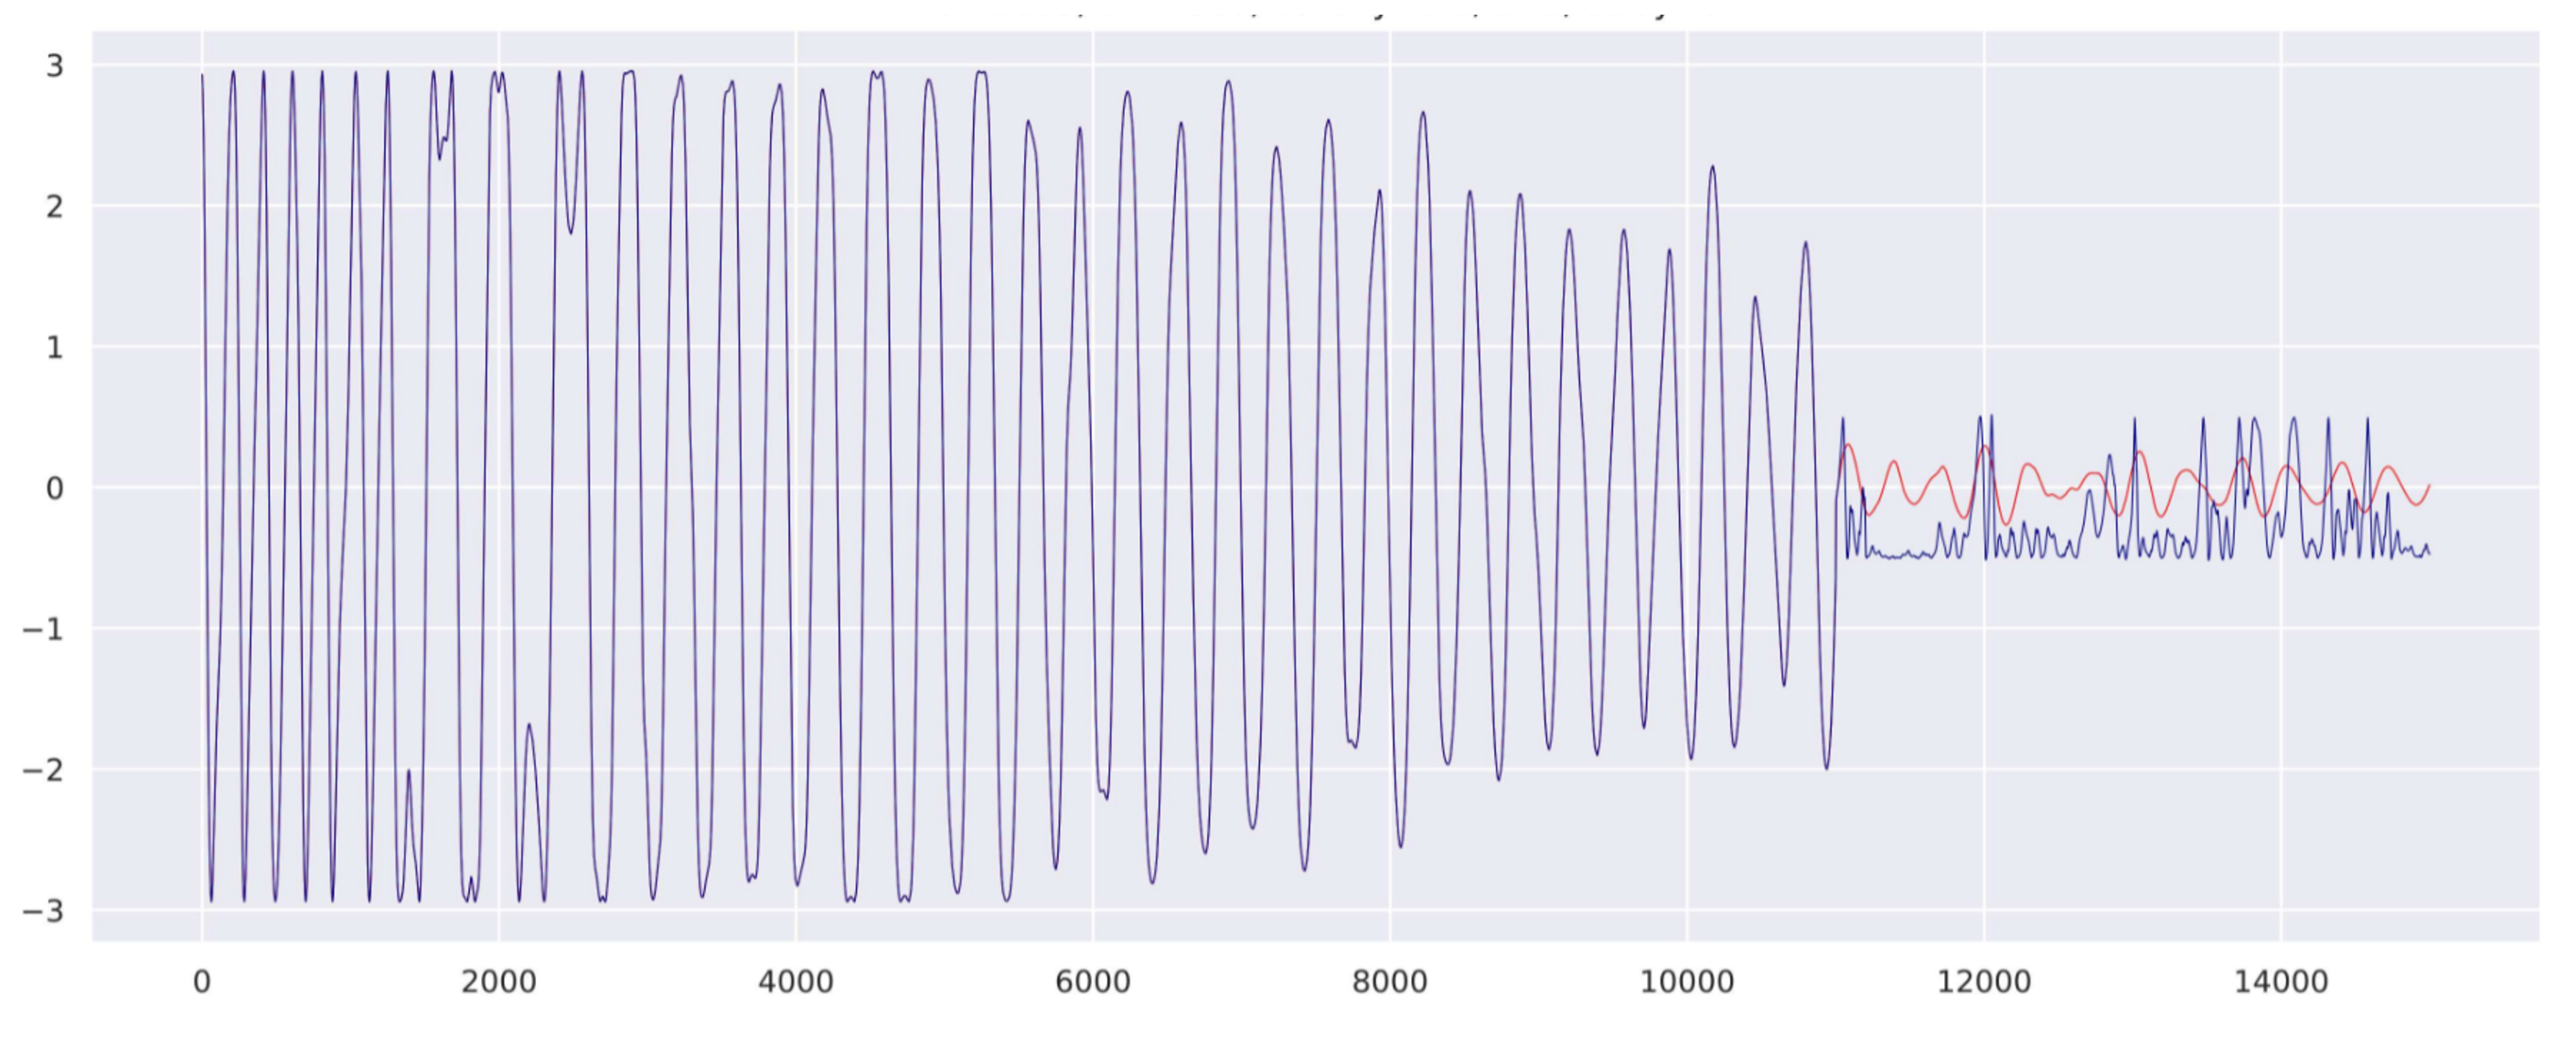
\includegraphics[scale=0.3]{Graphs/_dpfail_nonsurj.eps}
  \centering
\caption{Failure to forecast or learn a map which is not surjective: Evolution of the $y$-coordinate of the bottommost pendulum plotted here for 15000 timesteps. Plotted here the predicted value (red) versus the actual value (blue). The plots overlap for the first 10000 steps, the duration of training to learn the map $\Gamma$. Parameter-values are exactly as in the successful case discussed in the paragraph directly afterwards. Afterwards, the trajectories start diverging and it the predicted value no longer accurately represents the complexity or energy-loss of the actual data. }
\label{fig:dp_notsurjective}
\end{figure}
% \ednote{Can I say in the caption \emph{Parameter-values are exactly as in the successful case discussed in the paragraph directly afterwards.}}


Having spent ample time to discuss the challenges, we now change tone so as to satisfy the optimist and present a successful run of the DP-data to predict the future movement of the pendulum.

The system was driven for 15500 steps, of which the first 500 were immediately discarded to simulate the network `forgetting'. 
Input and reservoir matrices of the driven system $g$ were implemented as sparse matrices filled to 20\%. Parameter-values of $\alpha=0.99$ and $a=0.5$ were used.
The remaining 15000 datapoints were used to train a network with 128 neurons. 
The network was initialised to contain 16 hidden layers each with layer dimension 64 and activated with the $\tanh$ activation function.
Training was accomplished using 256 epochs with batch sizes 128. See Fig.~\ref{fig:dp_success_traj} for results pertaining to the trajectory taken component-wise from the DP's and then Fig.~\ref{fig:dp_success_density} to witness associated densities of predicted versus actual values.

\begin{figure}[ht]
  \centering
  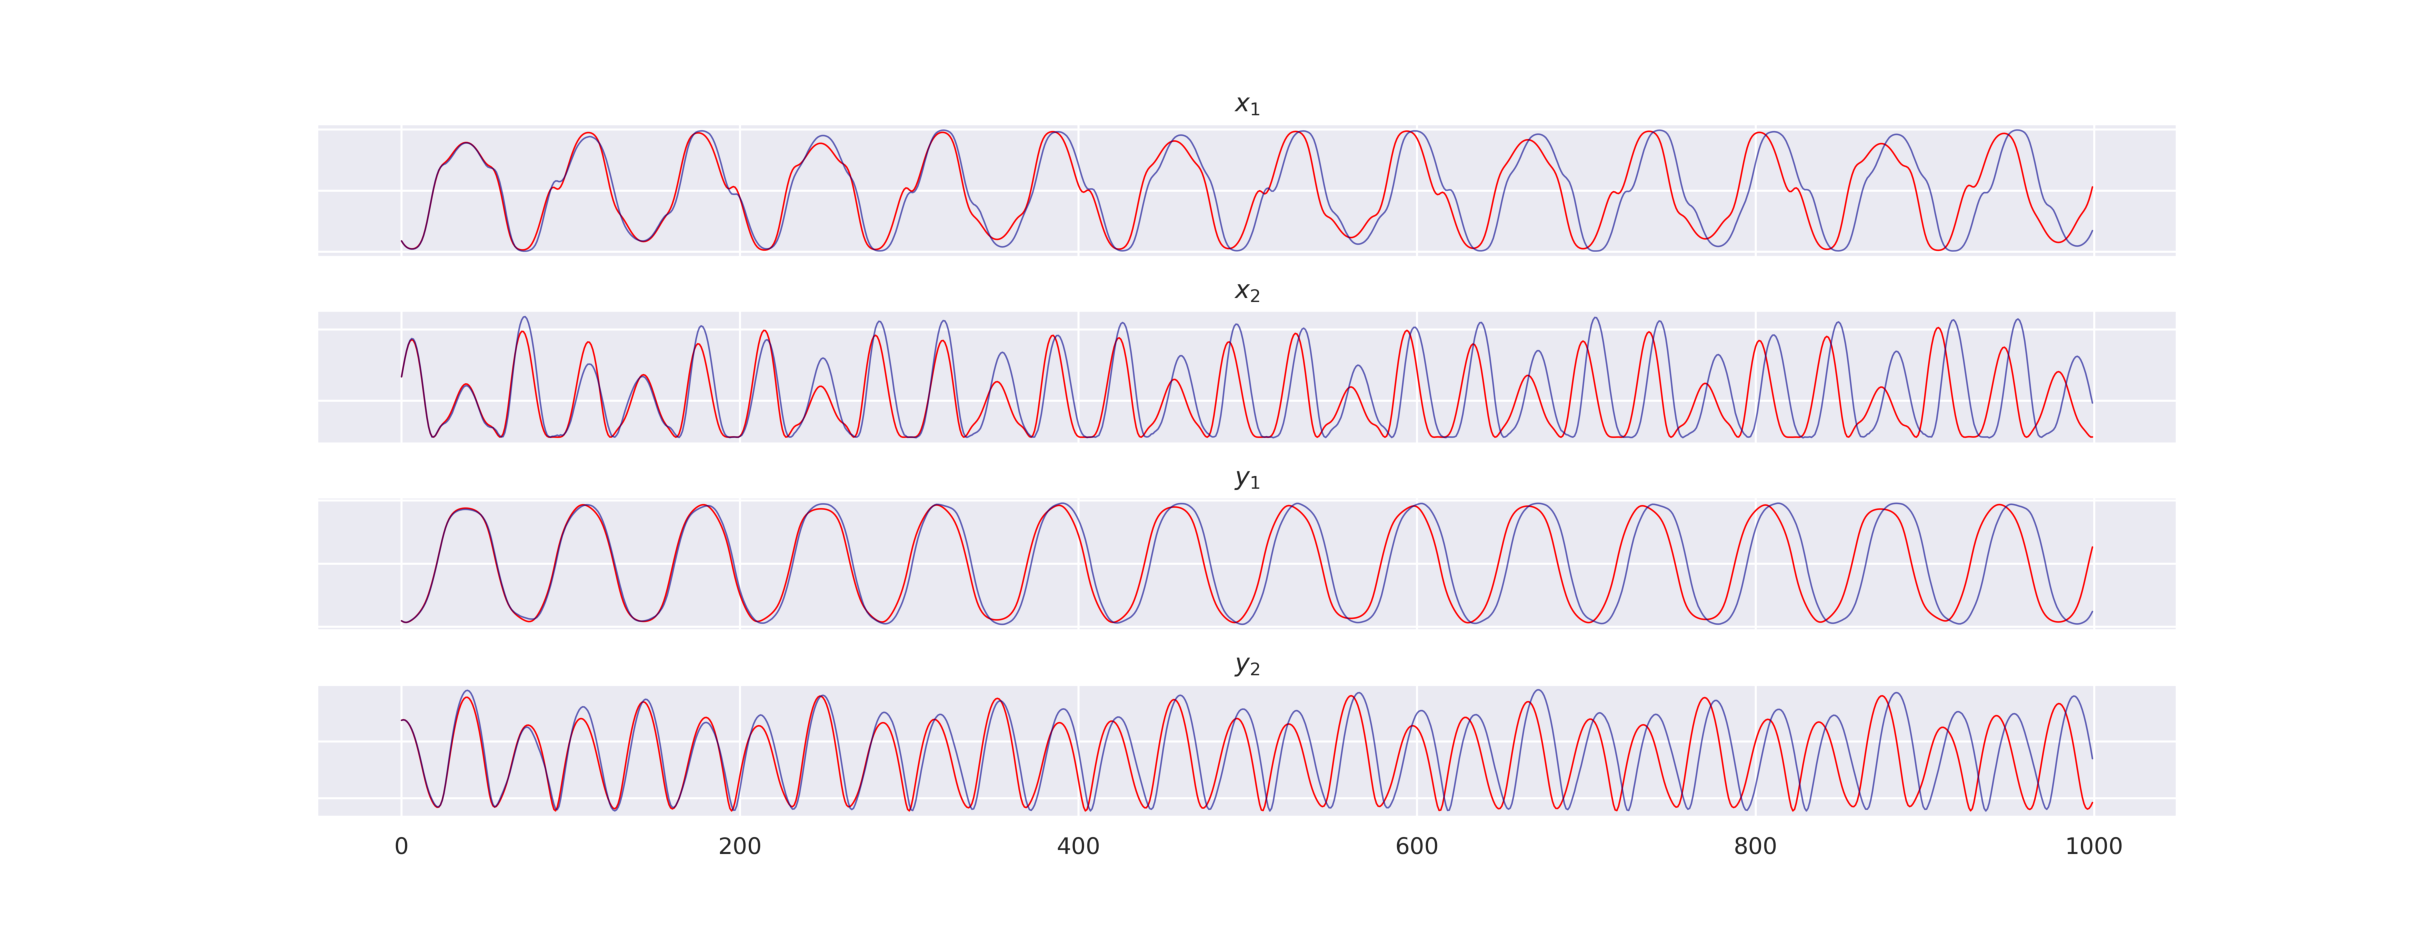
\includegraphics[width=0.95\linewidth]{Graphs/_dp_success_4coords_traj.eps} 
  \captionof{figure}{Predicted (red) and actual (blue) trajectories of the $x$- and $y$-coordinates of each of the pendulum heads. From top to bottom are as follows: $x$-coordinate of topmost pendulum head, $y$-coordinate of topmost pendulum head, $x$-coordinate of lower pendulum head, $y$-coordinate of lower pendulum head. 
  These graphs were constructed by predicting the DP 1000 timesteps into the future and in so doing illustrating the long-term consistency and accuracy of the learnt system. Here we lock onto the near-exact trajectory for about 300 timesteps and stay close up until about 600 seconds.  } 
  \label{fig:dp_success_traj}
\end{figure}
\begin{figure}[ht]
  \centering
  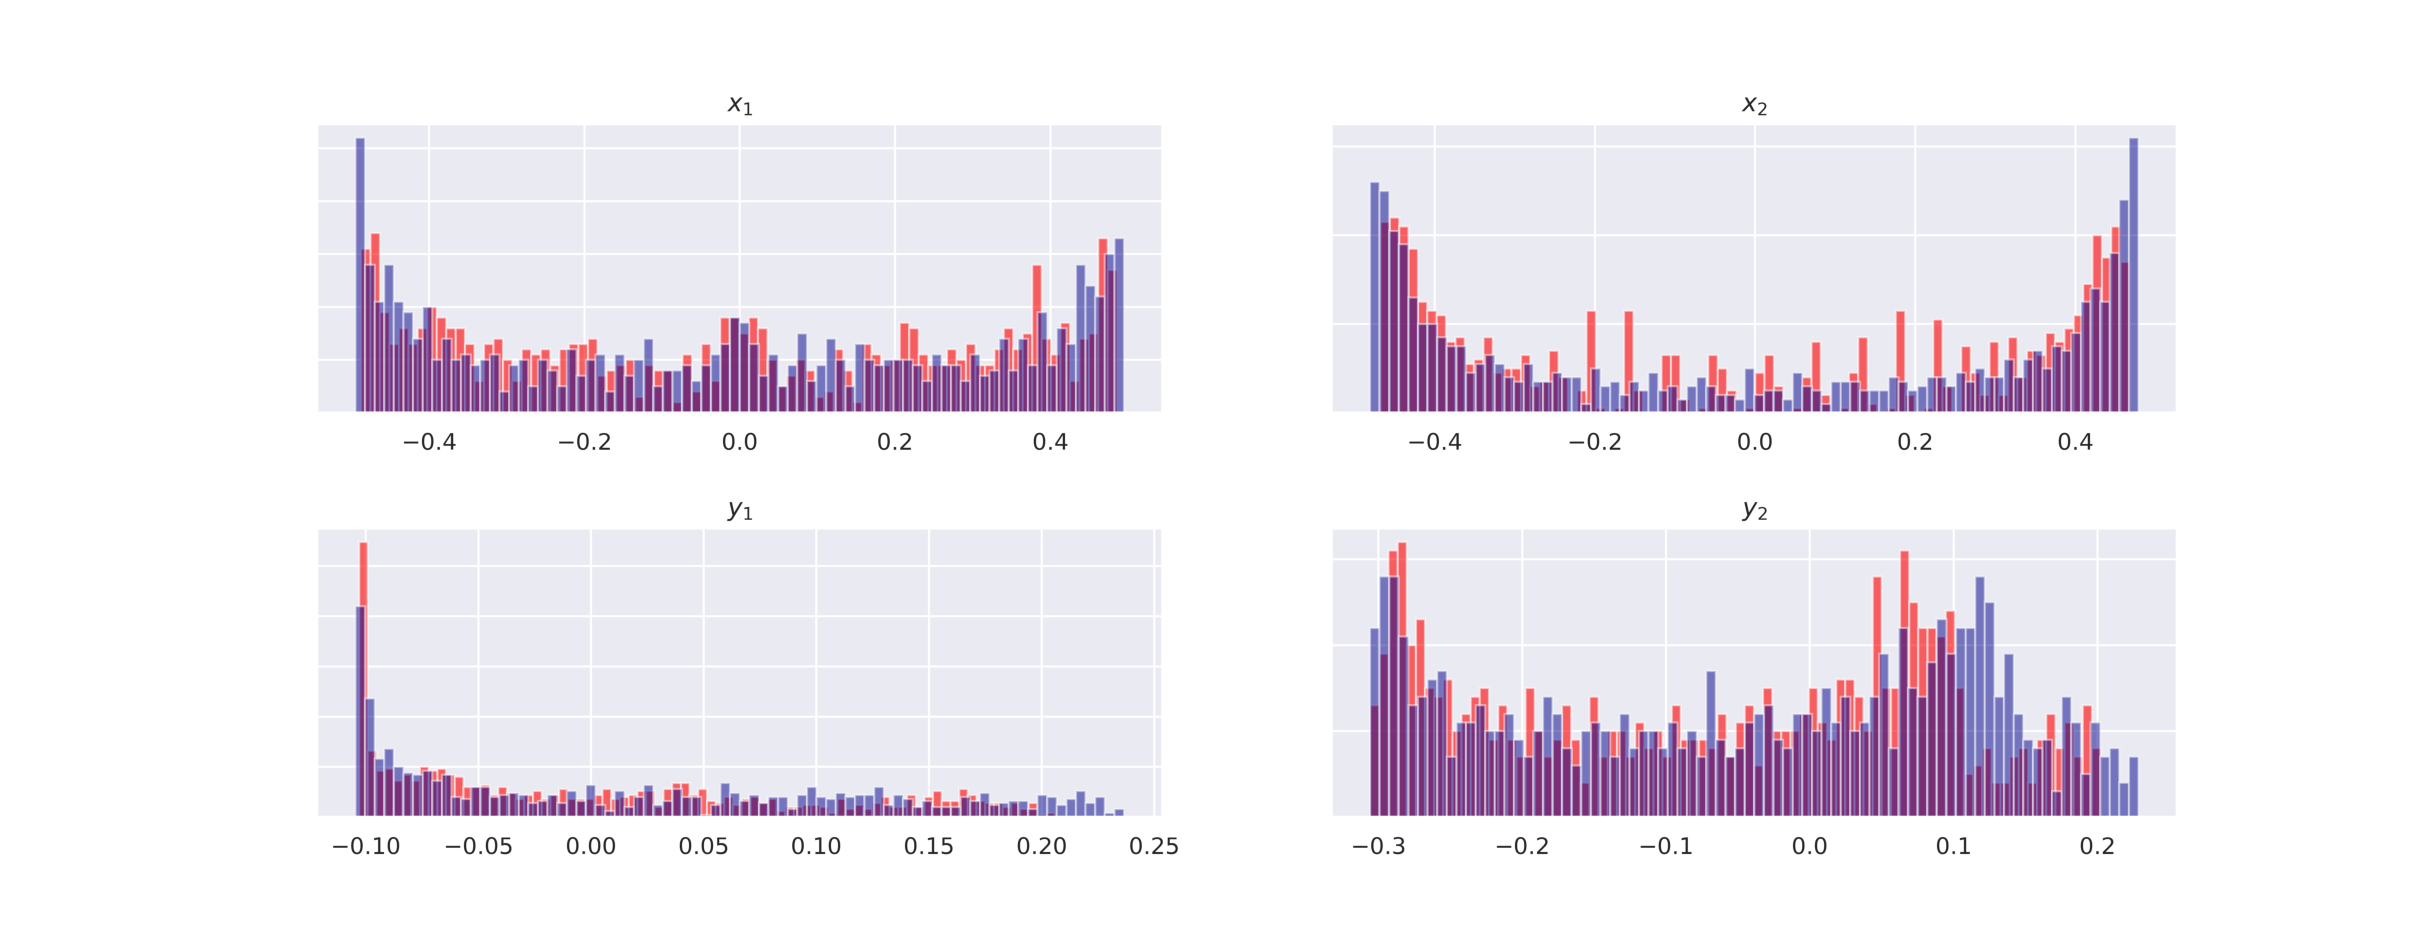
\includegraphics[width=\linewidth]{Graphs/_dp_success_4coords_hist.eps}
  \captionof{figure}{Densities of predicted and actual values of $x$- and $y$-coordinate of pendulum heads.}
  \label{fig:dp_success_density}
 \end{figure}
  

We now consider an experiment where noise is added to the system and find it to be incredibly robust. Employing the same parameters as in the preceding experiment, we include noise from a normal-distribution with zero mean value and standard deviation equal to 0.1 which equates to a signal-to-noise ratio of 39dB.

For the signal-to-noise ration we adopt the formula $\text{SNR}_{dB}=10\text{log}_{10}\big(\frac{P_\text{{signal}}}{P_{\text{noise}}}\big)$ where $P_\text{{signal}}$ refers to the variance observed in the normalised data and $P_{\text{noise}}$ represents the variance of the added noise.
Once again we display the actual and predicted trajectories for the noisy DP data in Figure~\ref{fig:noisydp_success_traj}. 
Next we consider the densities of the predicted and actual values in Figure~\ref{fig:noisydp_success_density} and observe that they display highly similar distributions.

\begin{figure}[ht]
  \centering
  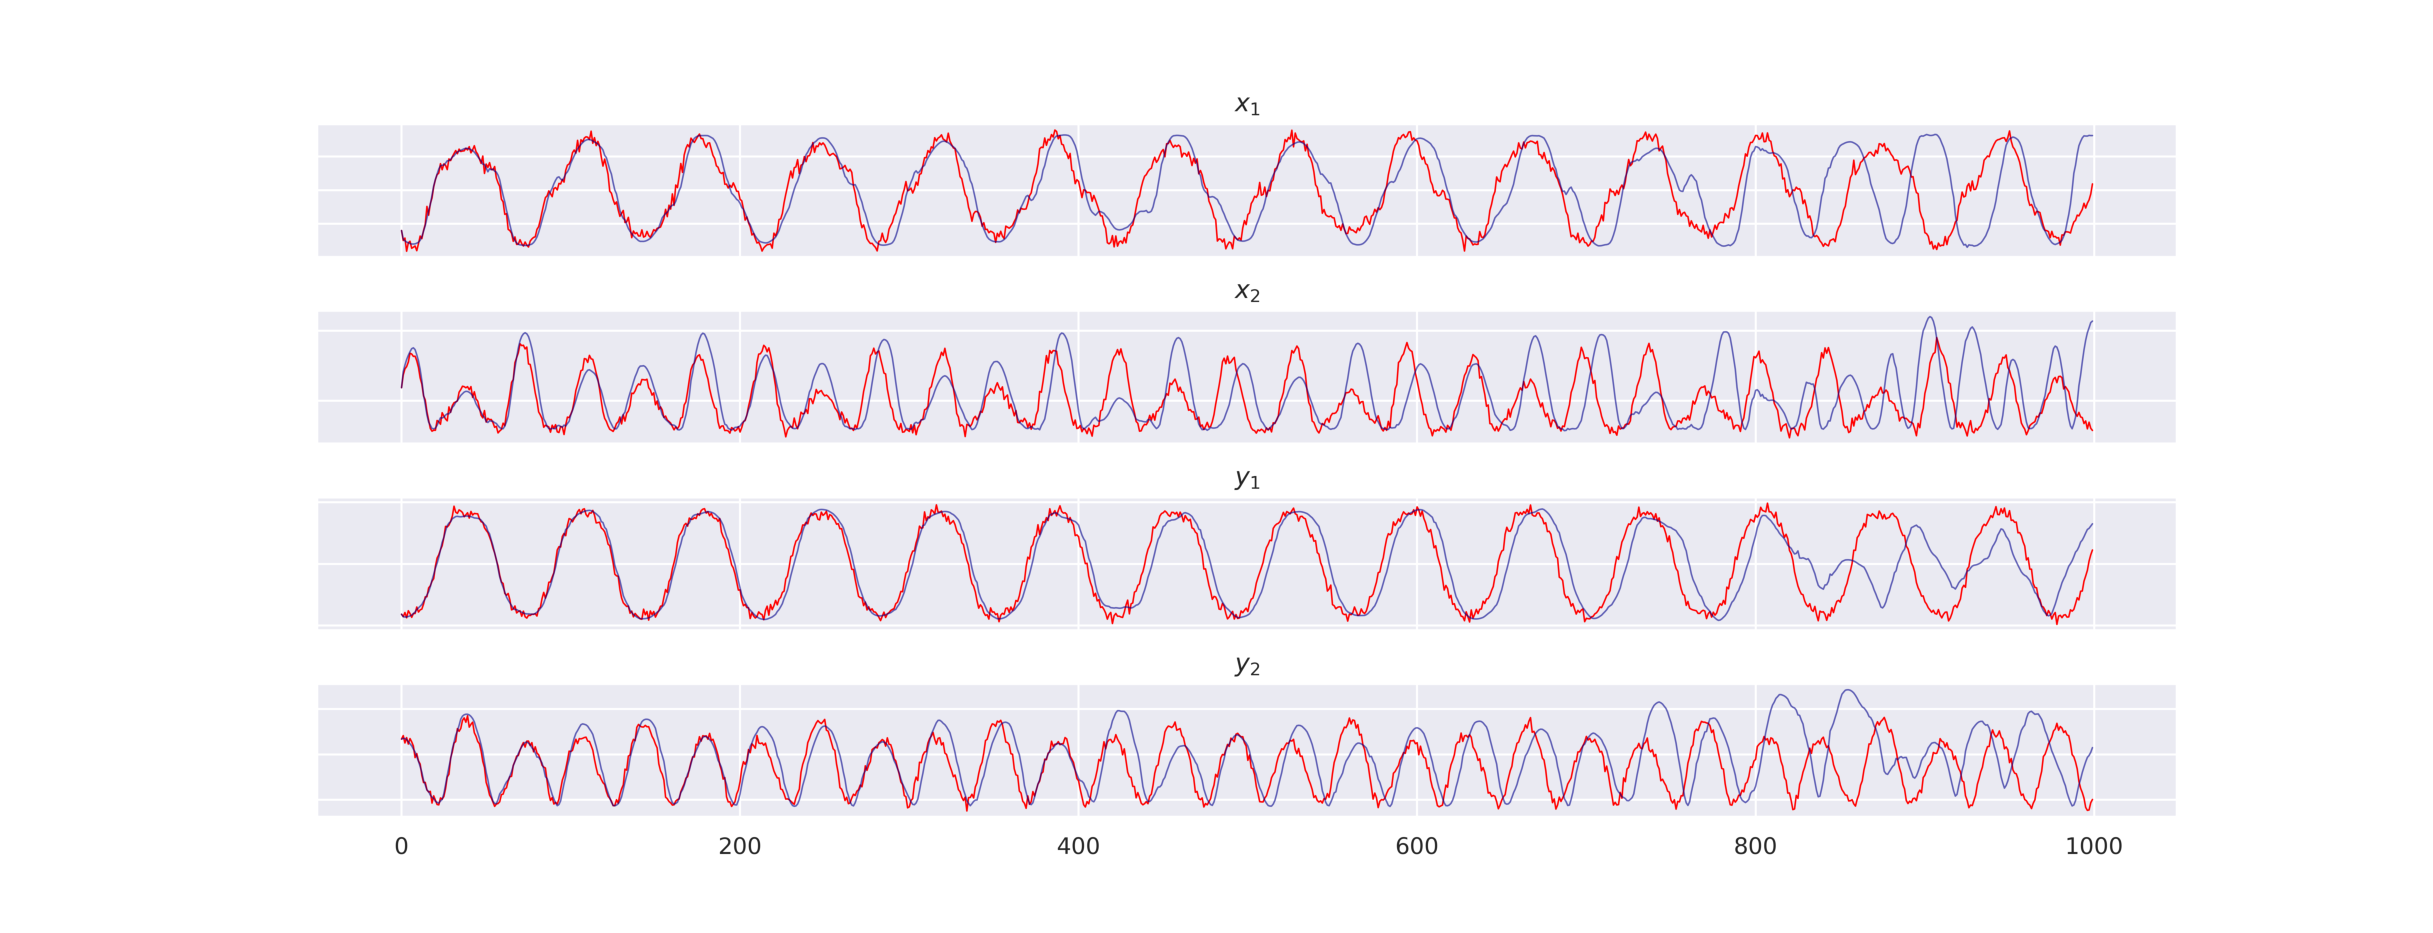
\includegraphics[width=0.95\linewidth]{Graphs/_dp_noise_FigCD_2030.eps} 
  \captionof{figure}{Predicted (red) and actual (blue) trajectories of the $x$- and $y$-coordinates of each of the pendulum heads with noise added from a normal distribution with mean zero and standard deviation 0.1, equating to approximately 39dB's of noise.
  These graphs were constructed by predicting the DP 1000 timesteps into the future and in so doing illustrating the long-term consistency and accuracy of the learnt system. Here we lock onto the near-exact trajectory for about 250 timesteps and stay close up until about 400 seconds.  } 
 \label{fig:noisydp_success_traj}
\end{figure}
\begin{figure}[ht]
  \centering
  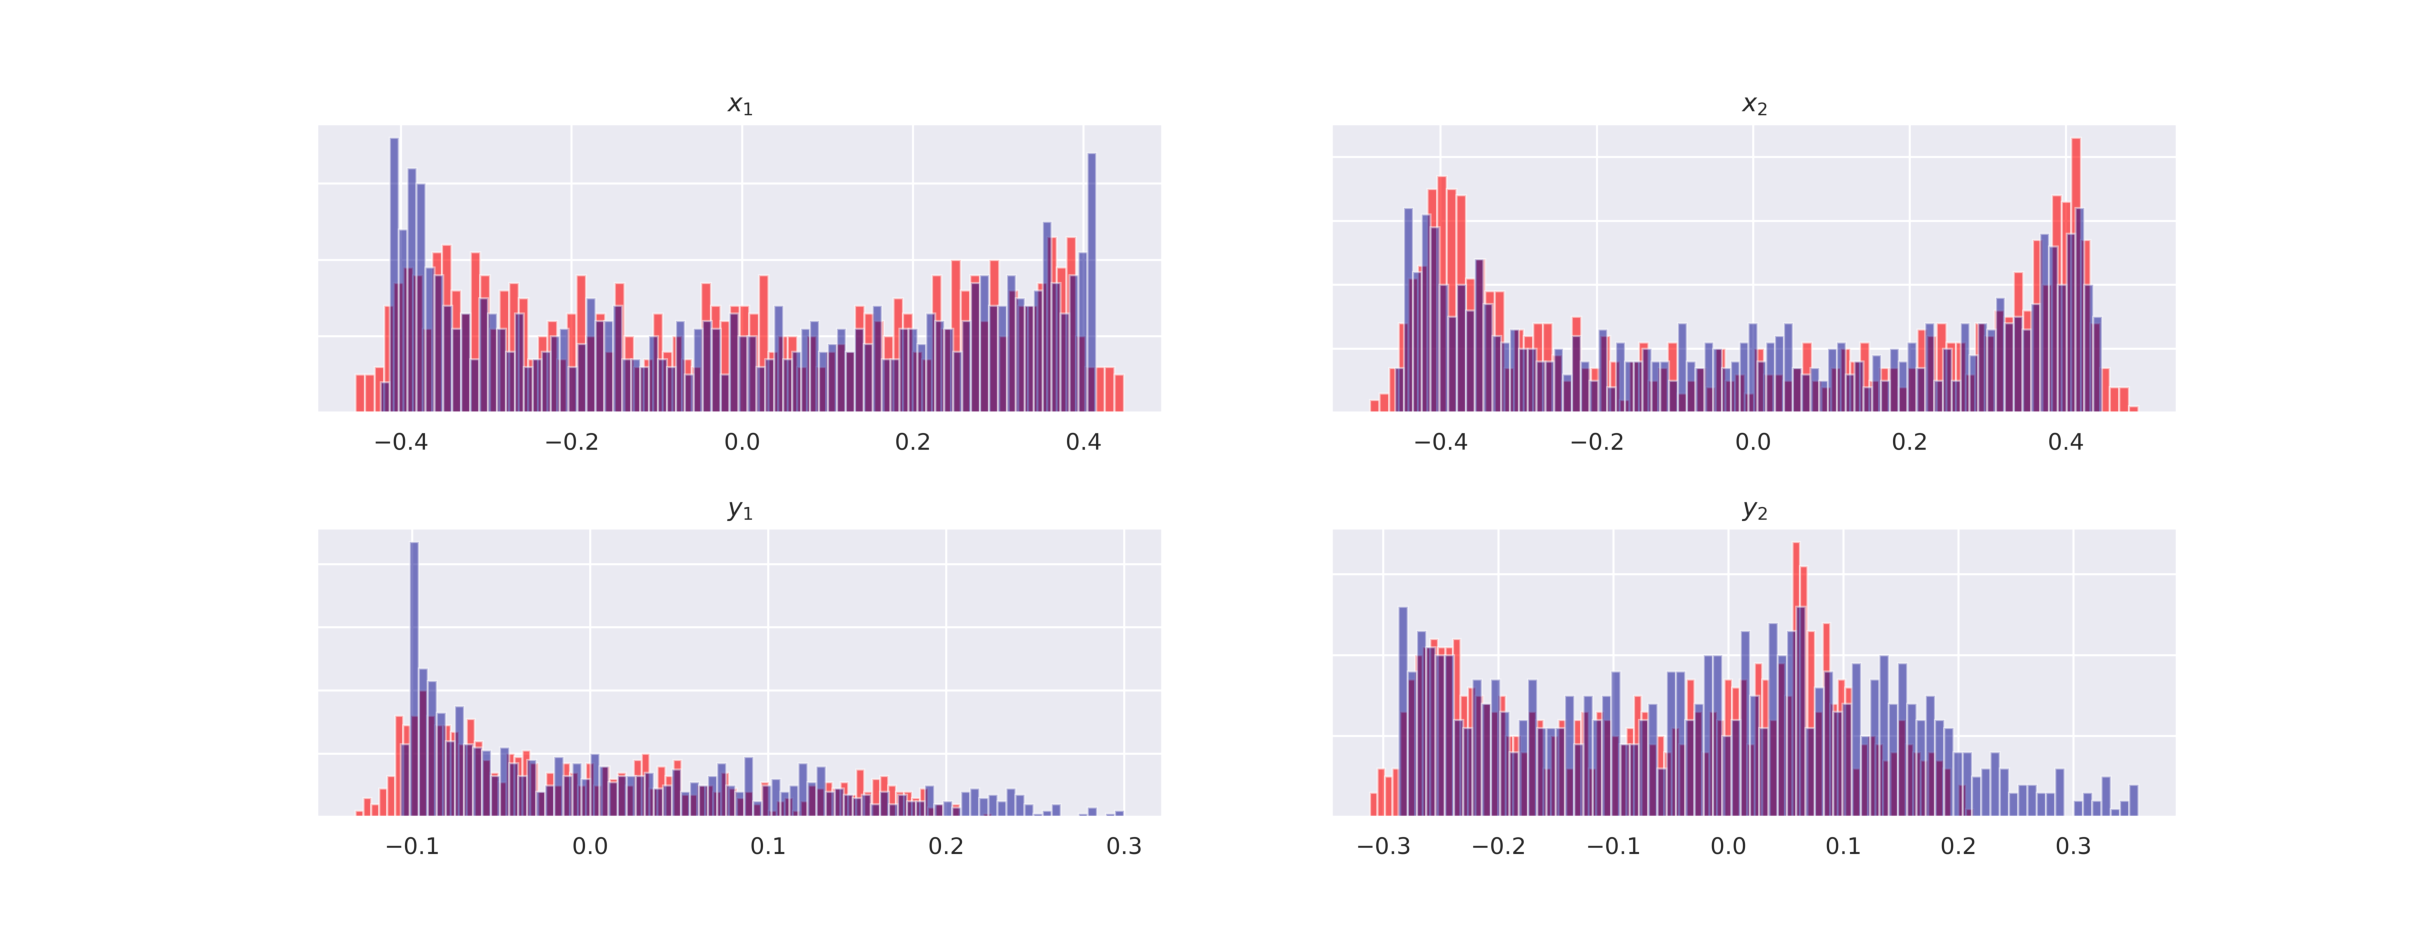
\includegraphics[width=\linewidth]{Graphs/_dp_noise_2B_2030.eps}
  \captionof{figure}{Densities of predicted and actual values of x-coordinate of first pendulum head.}
  \label{fig:noisydp_success_density}
 \end{figure}

%  Lastly, a run was done where only a single coordinate (the $y$-coordinate of the lower pendulum head) was fed into the system and we can illustrate through the obtained success that the coordinate contains all the information in its past states necessary to forecast its future evolution.
%  \textbf{Insert graphs here. Had to quickly change something here.}
 

\subsection{Additional Attractors: Clifford \& Thomas}
We follow the methodology presented in~\cite{manjunath2021universal} but opt to consider attractors different from the Lorenz system and H\'enon map for this project.

\subsubsection{Thomas' Cyclically Symmetric Strange Attractor}\label{Thomas_Attractor}
Thomas' Cyclically Symmetric Strange Attractor, a 3D attractor proposed in 1999 by Ren\'e Thomas in~\cite{ThomasAttractor}, is described by a set of three equations which is distinctly reminiscent of another deterministic three-equation model exhibiting chaotic behaviour proposed by Lorenz. 
It has a single parameter $\beta$ and has been shown to transition to chaotic behavious when $\beta<0.208186$~\cite{Thomas_BetaParameter}.
\begin{eqnarray}\label{eqns_thomas}
  x_{n+1} = \sin(y_n) - \beta{x_n} \\
  y_{n+1} = \sin(z_n) - \beta{y_n} \\
  z_{n+1} = \sin(x_n) - \beta{z_n}.
\end{eqnarray}

The behaviour of the system with a $\beta$-parameter value of 0.1056 was simulated by scaling the data generated from the equations to fall inside the interval $[-1,1]$. Two cases were considered: one noise-free and another perturbed by noise. 
Noise was generated  by adding data points taken from a normal distribution with a mean of zero and standard deviation 0.05, which translates approximately to a signal-to-noise ration of 33dB. 
$\text{SNR}_{dB}$ is calculated exactly as for the DP-data.

A sequence of 3000 observations in both the clear and noisy data-sets respectively was fed into the system with 300 entries discarded to simulate the network's loss of memory. 
The next 9000 steps were predicted and compared with true data. See Figure~\ref{fig:Thomas_trajectories} for the actual and predicted trajectories of the noise-free and perturbed systems respectively. 

\begin{figure}[ht]
  \centering
  \minipage{0.5\linewidth}
    \centering
    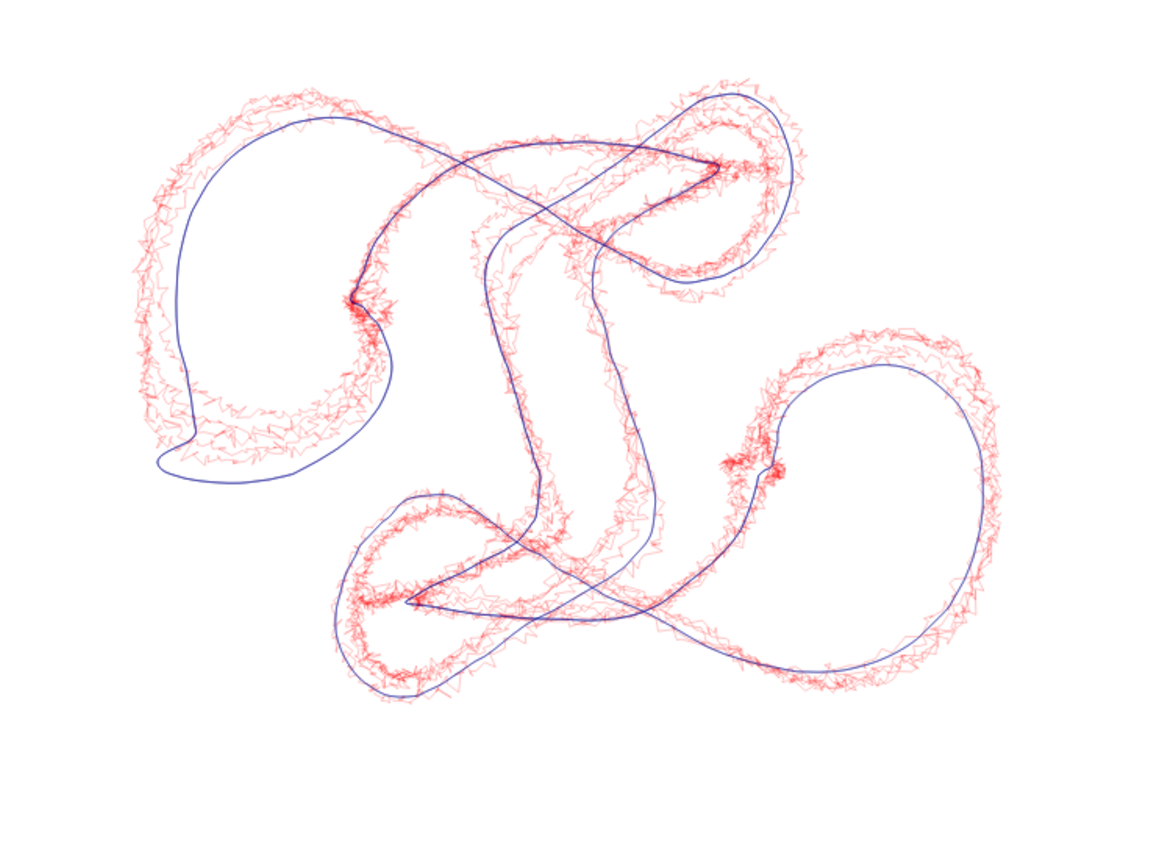
\includegraphics[width=0.8\linewidth]{Graphs/_thomas_noisy_0.1056.eps}
  \endminipage\hfill
  \minipage{0.5\linewidth}
    \centering    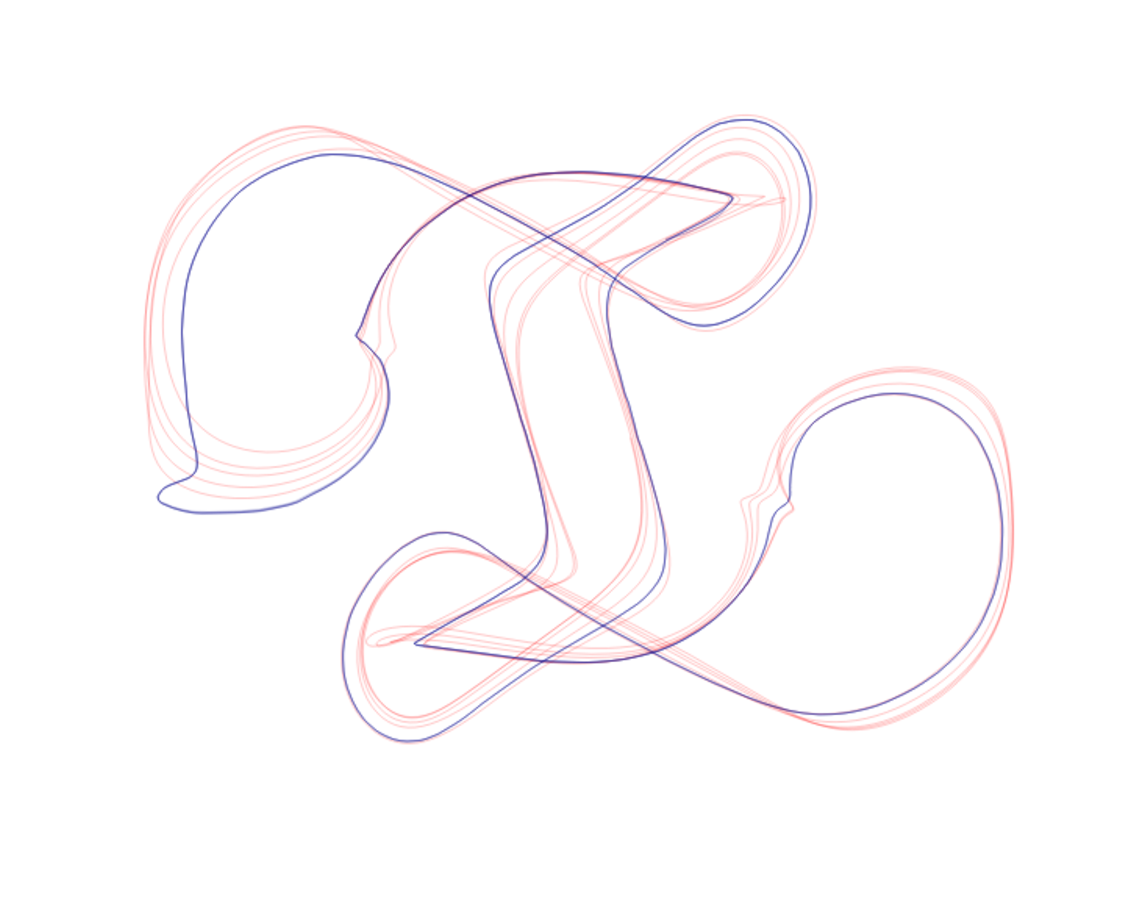
\includegraphics[width=0.8\linewidth]{Graphs/_thomas_clean_0.1056.eps}
  \endminipage
 \captionof{figure}{True (red) and predicted (blue) trajectories for the Thomas attractor with parameter value $\beta=0.1056$.Left: Noise added from normal distribution with mean zero and standard deviation 0.05. Right: No noise added to dataset.}
\label{fig:Thomas_trajectories}
\end{figure}


The RNN was initialised as follows: the dimension of the network is set equal to 500 neurons and 12 hidden layers of dimension 64 each were initialised. Training is realised through 150 epochs of batch sizes of 128 each; the map is learnt via the Adam Optimiser using finer and finer learning rates (0.001 and then divided by 10 at every iteration).

\begin{figure}[ht]
  \centering
  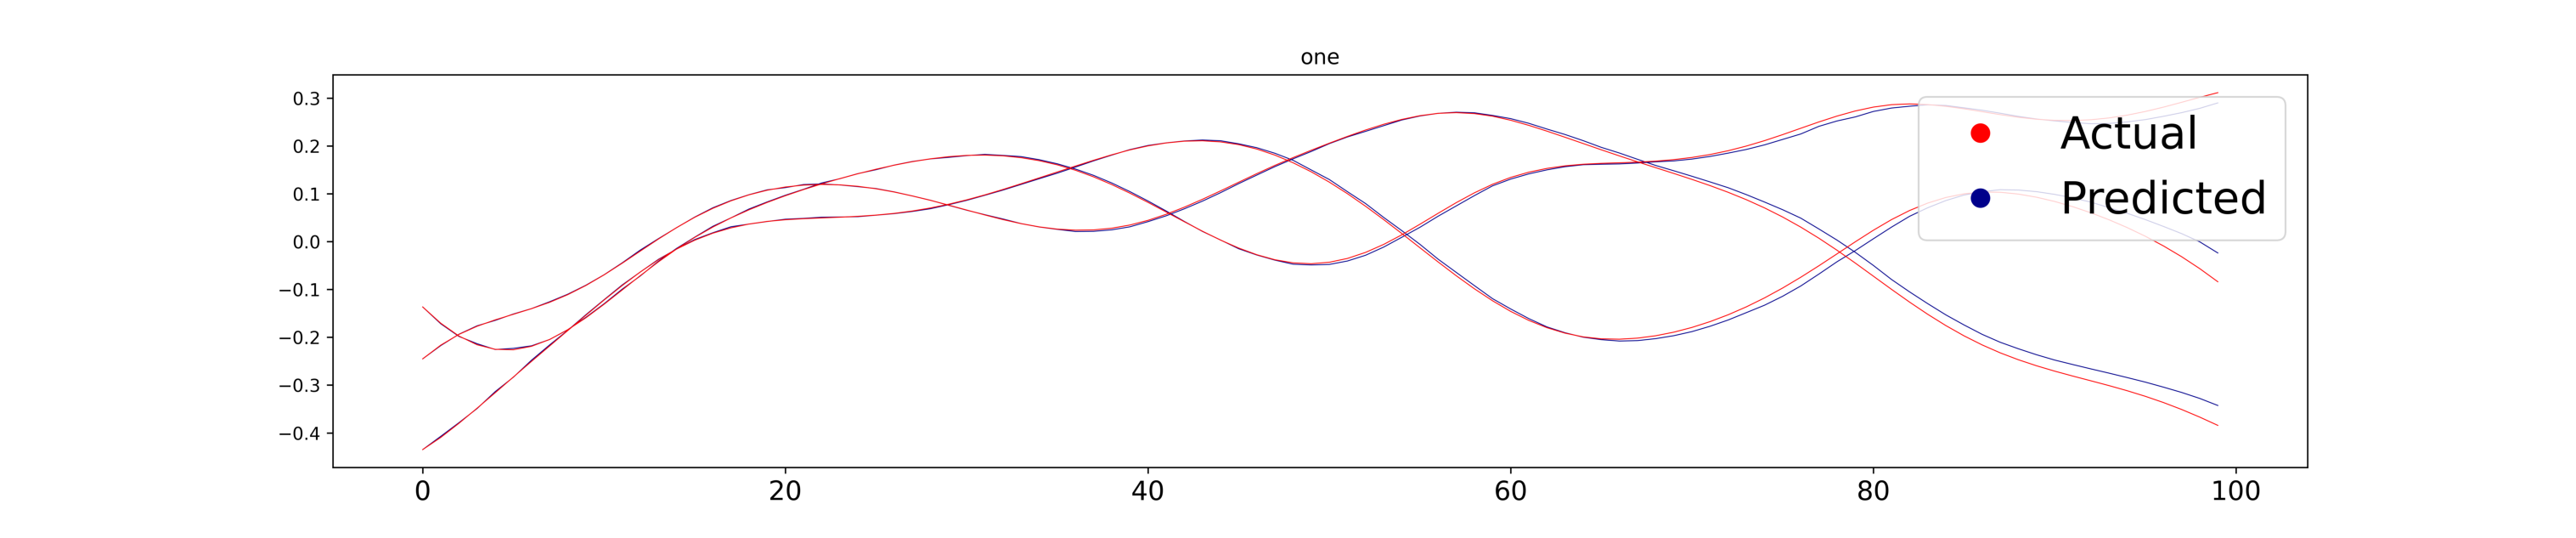
\includegraphics[scale=0.35]{Graphs/_Thomas_1.eps}\caption*{Predicted trajectories of the $x$- and $y$-coordinates for the Thomas attractor with parameter-value $\beta=0.1056$ demonstrate empirically the ability to predict the evolution of the trajectory for the next an estimated 100 timesteps into the future near-exactly. Here no noise was added.}
  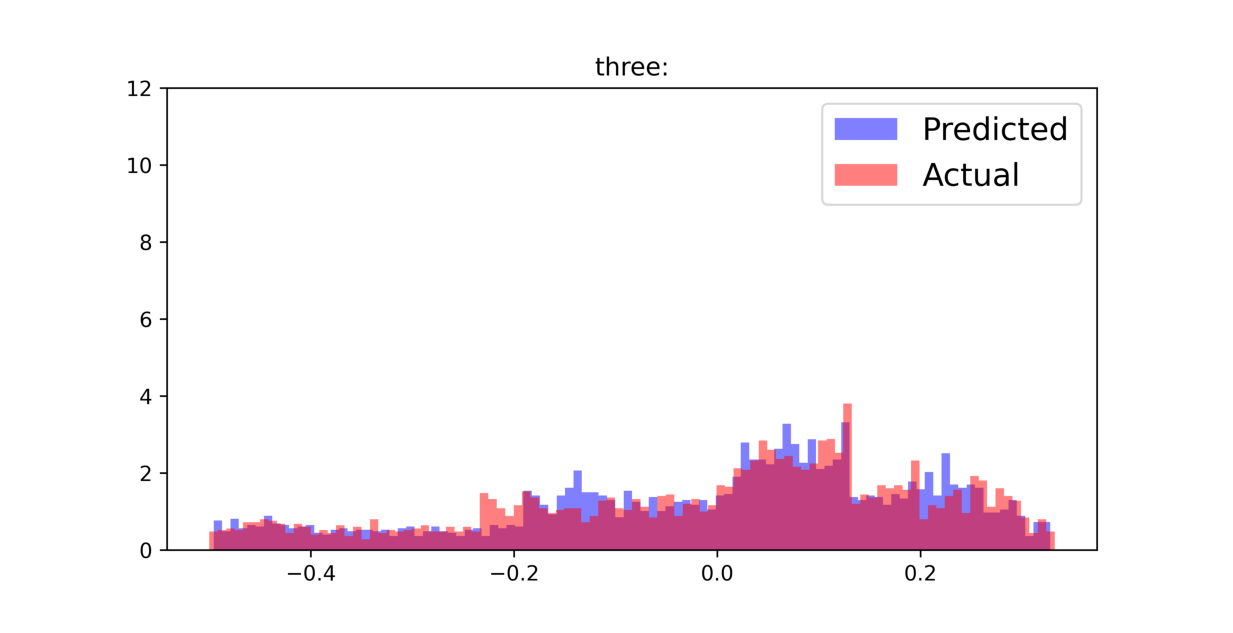
\includegraphics[scale=0.5]{Graphs/_Thomas_3.eps}\caption*{Represented here the learnt (blue) and actual (red) densities of the first coordinate ($x$-coordinate) of the dataset for the Cyclically Symmetric Attractor with parameter-value $\beta=0.1056$.}
\end{figure} \label{fig:Thomas_TrajDensity}


\subsubsection{Fractal Dream Attractor}

A finaldiscrete-time map named the Fractal Dream Attractor -- more commonly as the Pickover or Clifford Map (first discovered by Clifford A. Pickover and discussed in his fascinating book ``Chaos in Wonderland" \cite{PickoverChaos}) -- was also considered.
\begin{eqnarray}\label{eqns_clifford}
  {x_{n+1}=\sin(ay_n) + c\cos(ax_n)} \\
  {y_{n+1}=\sin(bx_n)+d\cos(by_n)}.
\end{eqnarray}


The behaviour of the system with a parameter values of $x_0=0$, $y_0=0$, $a = -1.7$,  $b = 1.8$, $c = -1.9$ and $d = -0.4$ was examined. 
Data was scaled to fit inside the interval $[-1,1]$. Only the noise-free case was investigated. 
Depictions of the empirical results are available in Figure~\ref{fig:Clifford}.
 A sequence of 25000 observations was fed into the system with 15000 entries discarded. 
 The reason for such a great number of discarded entries is the following: the system seems to have an incredibly long transient;driving it for less than 5000 entries only gives an accurate prediction to about 5 seconds and it starts improving when the discard is in the range $[10000,15000]$ to simulate the network's loss of memory. The next 1000 steps were predicted and compared with true data.


\begin{figure}[ht]
  \centering
  
\includegraphics[width=1.0\textwidth,left]{Graphs/_Clifford_1_nonoise.eps}
  \caption*{These graphs were constructed by predicting the Clifford system 1000 steps into the future and in so doing illustrating the long-term consistency and accuracy of the learnt system. As perceived here, we are able to lock on to the trajectory of the Clifford map almost exactly for the first 25 steps.}
  \minipage{0.5\textwidth}
      \centering
      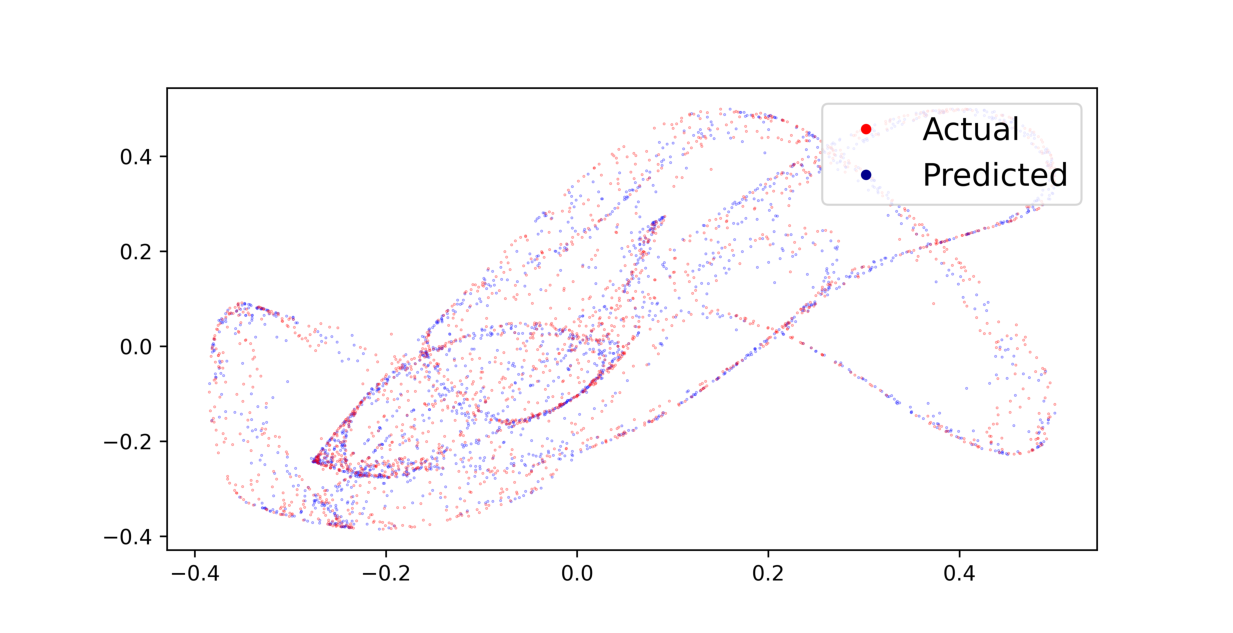
\includegraphics[width=\linewidth]{Graphs/_Clifford_2_nonoise.eps}
  \endminipage\hfill
  \minipage{0.5\textwidth}
    \centering
    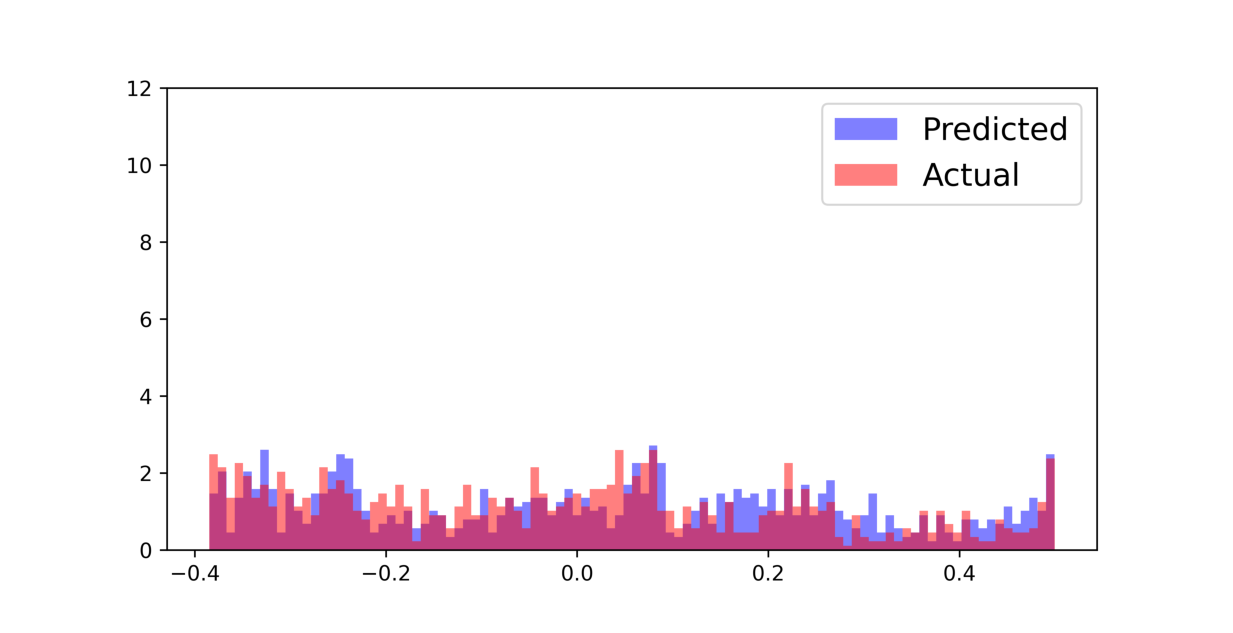
\includegraphics[width=\linewidth]{Graphs/_Clifford_3_nonoise.eps}
  \endminipage
  \caption{The bottom row, left, shows a plot of the true attractor (red) and the predicted values (blue). Bottom row, right, shows the distribution of the first coordinate of the learnt system (blue) and the actual Clifford system (red). }
  \label{fig:Clifford}
\end{figure}

 The RNN was initialised exactly as for Thomas' Cyclically Symmetric Strange attractor: the dimension of the network is set equal to 500 neurons and 12 hidden layers of dimension 64 each were initialised. Training is realised through 150 epochs of batch sizes of 128 each; the map is learnt via the Adam Optimiser using finer and finer learning rates (0.001 and then divided by 10 at every iteration).

\section{Functional Complexity Reduction in Noninvertible Maps}
The map $G_T : Y_T \to Y_T$ is a homeomorphism since it is conjugate to the homeomorphism $\widehat{T}$ even though $T$ may be a non-invertible map. We remark that in the case of a non-invertible map, empirically it is found that $G_T$ is much more linear than $T$ as measured by what is called the multidimensional correlation coefficient $\rho$. This amplification in linearity  or the increased value of the multidimensional correlation coefficient $\rho$  is also true for invertible maps and we refer to empirical results in \cite{Supp}. Here we consider only one non-invertible map pertaining to the Clifford attractor to add to the results in \cite{Supp}. This coefficient is a generalization of the Pearson correlation coefficient for real-valued random variables to random vectors (e.g., \cite{puccetti2019measuring}). We state the details of computing this coefficient between 
$(x_{n-1},x_n)$ and $G_T(x_{n-1},x_n)$. 
If $\Sigma_{a}$ and $\Sigma_{b}$ denotes the covariance matrices of the vectors $(x_{n-1},x_n)$ and $G_T(x_{n-1},x_n)$ respectively, and if $\Sigma_{ab}$ denotes the covariance matrix between the vectors $(x_{n-1},x_n)$ and $G_T(x_{n-1},x_n)$, then the multidimensional correlation coefficient is computed by using the traces of these matrices.
\[
    \rho= \frac{\text{tr}({\Sigma_{ab}})}{\text{tr}({\sqrt{\Sigma_a\Sigma_b}})}.
\]
This multidimensional correlation coefficient satisfies one of the desired and well-known properties of the one-dimensional Pearson coefficient. That is, $\rho=\pm 1$ if and only if $Y\overset{d}{=}AX+b$ for some invertible matrix $A$ and vector $b$. Hence $\rho$, and in practice can be used  to measure the linear relationship between two random vectors of the same dimension and thus serves as an indicator of functional complexity. For the non-invertible system defined by the Clifford attractor, we indicate the difference by which $\rho$ changes for $G_T$ in Table~\ref{tbl_attractorsPearson}.
Following~\cite{manjunath2021universal}, we say that this multidimensional correlation coefficients $\rho$ to evidence a general reduction in the functional complexity of the map $G_T$ emerging due to a RNN. In the 
Table~\ref{tbl_attractorsPearson}, the second column corresponds to the amount of artificial neurons (the dimension of $X$) in the implemented RNN.
               
% \begin{center}
  \begin{table} 
      \scalebox{0.65}
      \centering
      {\begin{tabular}{|c|c| c c |} 
          \toprule
          Input & Dimension of $X$ & $u_n$ vs $u_{n+1}$ 
          & $\begin{bmatrix}
              x_{n-1}\\
              x_n
          \end{bmatrix}$ vs $\begin{bmatrix}
              x_n\\
              x_{n+1}
          \end{bmatrix}$ \\
          \midrule      
          % \hline
          % $(w_n)$ is the Lorenz states, sampled every 0.1 timestamps. & & &\\
          % \multirow{3}{*}{$u_n=\frac{1}{100}w_n$} & 10 &0.9311  & 0.9731\\
          %     & 100 &  & 0.9934\\
          %     & 1000 & & 0.9930\\              
          % \multirow{3}{*}{$u_n=\frac{1}{10}(\sin(0.1w_{n,x})+\sin(0.1w_{n,y})+\sin(0.1w_{n,z}))$} 
          %     & 10 &0.8401  & 0.9392\\
          %     & 100 & & 0.9616\\
          %     & 1000 & & 0.9737\\
          % \hline         
               \midrule  
               $(w_n)$ comes from the Clifford Attractor \\ (for $a = -1.7; b = 1.8; c = -1.9; d = -0.4$): & & & \\
        {$w_{n+1}= \begin{bmatrix} \sin(aw_{n,y}) + c\cos(aw_{n,x}) \\ 
                                                                    \sin(bw_{n,x})+d\cos(bw_{n,y}) \end{bmatrix}$} & & & \\
          \multirow{3}{*}{$u_n = w_n-\overline{w}$}
              & 10 & -0.21713 & 0.78719 \\
              & 100 & &  0.8334 \\
              & 1000 & & 0.84854 \\
          % \hline 
          % $(w_n)$ comes from the Logistic map: & & & \\
          % {$ w_{n+1}  = 4w_n(1-w_n)$} & & & \\
          % \multirow{3}{*}{$u_n = w_n - 0.5$} 
          %     & 10 &-0.0314  & 0.5577\\
          %     & 100 &  & 0.7150\\
          %     & 1000 & & 0.7826\\
          % \hline
          % \hline
          % $(w_n)$ comes from the Svensson Attractor \\ (for $a = -1.7; b = 1.8; c = -1.9; d = -0.4$): & & & \\
          % {$w_{n+1}= \begin{bmatrix} d\sin(aw_{n,x}) - \sin(bw_{n,y}) \\ 
          %                                                             c\cos(aw_{n,x})+\cos(bw_{n,y}) \end{bmatrix}$} & & & \\
          %   \multirow{3}{*}{$u_n = w_n-\overline{w}$}
          %       & 10 & -0.2243 & 0.49698 \\
          %       & 100 & &  0.63310 \\
          %       & 1000 & & 0.71151 \\
           \bottomrule
                \end{tabular}}\label{Table_FC}%\ednote{http://paulbourke.net/fractals/peterdejong/}
     \caption{
              Following~\cite{manjunath2021universal}, we determine the multidimensional correlation coefficients $\rho$ to evidence a general reduction in the functional complexity of the map $G_T$ emerging due to a RNN. Rows correspond to distinct dynamical systems considered in the experiments
              The second column corresponds to the amount of artificial neurons (the dimension of $X$) in the implemented RNN.
              The last two columns comprise numerical estimates of $\rho$ for the relevant vectors. The linear association between $u_n$ vs $T(u_{n})$, as well as the linear relationship 
              $\begin{bmatrix}
                x_{n-1}\\
                x_n
            \end{bmatrix}$ vs 
            $G_T 
            \left({\begin{bmatrix}
                x_{n-1}\\
                x_n
            \end{bmatrix}}\right)$ 
              may be contrasted by the reader. 
              Finally, the RNN's dimension (from \eqref{Seq_RNN})
              is provided to exhibiting that an increase in dimension of the driven system will 
              typically result in a map $G_T$ with less functional complexity.}
      \end{table}\label{tbl_attractorsPearson}
% \end{center}

In summary, the numerical results not only corroborate the theory of employing the notion of causally embedding a dynamical system for data-driven modeling by showing both long-term topological consistency (the attractor reconstruction) and statistical consistency (the densities of the actual and predicted match).